% NeuroAgent / NeuroBench — paper plan for Nature Machine Intelligence (Article).
% Template: Springer Nature LaTeX template v3.1 (December 2024), option sn-nature, as linked from
% the NMI formatting guidelines. Build: `tectonic main.tex` in this folder (see ../README.md).
%
% This file is a plan, not the manuscript: every section states its role in the narrative, what
% goes in it, its structure and length, and the artefacts it needs. Prose comes later.

\documentclass[pdflatex,sn-nature]{sn-jnl}

\usepackage{graphicx}
\usepackage{amsmath,amssymb}
\usepackage{booktabs}
\usepackage{tabularx}
\usepackage{needspace}
\usepackage{xcolor}
\usepackage{enumitem}
\graphicspath{{../figures/}}
\setlist{nosep, leftmargin=1.2em}

\definecolor{cernblue}{HTML}{0033A0}
\definecolor{cernnavy}{HTML}{1C446A}
\definecolor{cernorange}{HTML}{E15E32}

% One block per section or subsection, always in this order.
\newcommand{\role}[1]{\par\smallskip\noindent\textcolor{cernblue}{\textbf{Role in the narrative.}} #1\par}
\newcommand{\content}{\par\smallskip\noindent\textcolor{cernblue}{\textbf{What goes here.}}\par}
\newcommand{\structure}{\par\needspace{10\baselineskip}\smallskip\noindent\textcolor{cernblue}{\textbf{Structure and length.}}\par}
\newcommand{\artefacts}{\par\needspace{8\baselineskip}\smallskip\noindent\textcolor{cernblue}{\textbf{Artefacts and why.}}\par}
\newcommand{\status}[1]{\par\smallskip\noindent\textcolor{cernorange}{\textbf{Status.} #1}\par}

% Placeholder for a display item that does not exist yet.
\newcommand{\figplaceholder}[2]{%
  \fcolorbox{cernnavy!60}{cernnavy!4}{\parbox{0.96\textwidth}{\small
    \textbf{#1}\par\smallskip #2}}}

\raggedbottom

\begin{document}

\title[Policy rewards for local diagnostic agents]{Executable clinical policies teach small open
models safe diagnostic work-ups}

\author*[1]{\fnm{Andrea} \sur{Protani}}\email{TODO}
\author[1]{\fnm{TODO} \sur{Supervisor}}
\author[2]{\fnm{TODO} \sur{Physician reviewer}}
\affil*[1]{\orgname{TODO affiliation}}
\affil[2]{\orgname{TODO clinical affiliation}}

\keywords{clinical AI agents, sequential diagnosis, reinforcement learning, process supervision,
verifiable rewards, local language models, neurology}

\maketitle

% Abstract plan: the narrative of the paper and what it must prove. The 150-word abstract is
% written last, one sentence per narrative move below.

\section*{Abstract (150 words, no references)}

\role{The whole paper in six moves; the reader must leave with the thesis and the central number.}

\content
\begin{itemize}
\item \textbf{Thesis.} A diagnostic agent a hospital can run is a small open model on local hardware;
it learns a safe work-up, not only the right answer, when it is trained on an executable,
physician-reviewed clinical policy instead of accuracy and cost.
\item \textbf{General claim for NMI readers.} Process rewards beat outcome rewards for agents in
high-stakes domains when the process is an executable specification experts can audit. Neurology
is the testbed.
\end{itemize}

\structure
\begin{enumerate}
\item \textbf{Constraint}: patient data cannot leave the hospital, so the agent is a 4--9\,B open model.
\item \textbf{Gap}: sequential-diagnosis benchmarks score outcome (accuracy, cost) and cannot tell a
safe work-up from a lucky or harmful one; as a reward, outcome invites shortcuts.
\item \textbf{Idea}: one executable policy per case, approved by two physicians, used as metric and as
RL reward.
\item \textbf{Resource}: NeuroBench, 600 cases, 20 conditions, 16 tools, [N] approved policies.
\item \textbf{Central result}: policy-reward RL vs outcome-reward RL, effect sizes, held-out conditions.
\item \textbf{Implication}: executable process rewards as a verifiable training signal.
\end{enumerate}

\artefacts
What we must prove, each claim with the experiment that tests it and the result that would refute it.\par\smallskip
\noindent{\small
\begin{tabularx}{\linewidth}{@{}>{\raggedright\arraybackslash}p{0.05\linewidth}>{\raggedright\arraybackslash}p{0.34\linewidth}>{\raggedright\arraybackslash}p{0.16\linewidth}>{\raggedright\arraybackslash}X@{}}
\toprule
& Claim & Evidence & Refuted if \\ \midrule
C1 & Outcome metrics hide unsafe and incomplete work-ups and change the ranking of models
   & E4, Fig.~3 & correct diagnoses rarely come with violations; Kendall $\tau\approx1$ \\
C2 & Policy-reward RL lowers safety violations and raises required coverage at equal accuracy,
     vs outcome-reward RL & E1, Fig.~4 & no paired difference, or accuracy drops \\
C3 & Physicians agree with the policy reward more than with accuracy+cost or an LLM judge
   & E2, Fig.~5 & $\rho_{\text{policy}}\le\rho_{\text{outcome}}$ \\
C4 & The gains hold on unseen conditions and on real records & E1 held-out, E3, Fig.~6
   & gain vanishes on held-out or MIMIC-IV \\
C5 & The agent runs on one GPU at a cost per case far below frontier APIs & E5, Fig.~6
   & latency or cost not compatible with use \\
\bottomrule
\end{tabularx}}
\par\smallskip
\textbf{Not claimed:} clinical readiness, superiority over physicians or frontier models,
generality beyond neurology. Never ``concurrent'' for SDBench.

\status{Every number waits for runs on the frozen dataset after the leakage fixes.}

% Overview: positioning, format limits, word budget, display items and risks. Thesis, narrative and
% claims are in the abstract plan.

\section*{Overview: positioning, budget, display items, risks}

\noindent\textbf{Positioning: what each line of prior work gives, and our delta}\par\smallskip
\noindent{\small
\begin{tabularx}{\linewidth}{@{}>{\raggedright\arraybackslash}p{0.27\linewidth}>{\raggedright\arraybackslash}p{0.33\linewidth}>{\raggedright\arraybackslash}X@{}}
\toprule
Prior work & What it gives & Our delta \\ \midrule
SDBench / MAI-DxO~\cite{nori2025sequential} & The sequential-diagnosis format; frontier models
  scored on accuracy and cost & Process-level, physician-auditable policy; used as reward for small
  local models. Prior art, never ``concurrent'' \\
Hager et al.~\cite{hager2024evaluation} on MIMIC-IV~\cite{johnson2023mimiciv} & Local models fail on
  real records and ignore guidelines & The training signal that targets that failure \\
AgentClinic~\cite{schmidgall2026agentclinic}, MedAgentBench~\cite{jiang2025medagentbench},
MedAgents~\cite{tang2024medagents} & Interactive benchmarks & They score outcome or use an LLM judge;
  no executable per-case policy; not rewards \\
Clinical RL (DiagGym, CDPR; TODO refs), GRPO~\cite{shao2024deepseekmath},
DAPO~\cite{yu2025dapo} & Outcome or cost-aware rewards & That reward is our outcome arm in E1 \\
Process supervision~\cite{uesato2022solving,lightman2024verify} & Process beats outcome in maths, with
  human or learned step labels & Process as a verifiable expert specification; stakes are safety \\
\bottomrule
\end{tabularx}}

\medskip
\noindent\textbf{NMI Article limits (checked 26 Oct 2026).} Main text $\le$3,500 words (without
abstract, Methods, references, legends); abstract $\le$150; $\le$6 display items; $\sim$50 references;
$\le$10 Extended Data items. Avoid: ``concurrent'', ``clinically deployable'', ``human-level'',
``solves''.

\medskip
\noindent
\begin{minipage}[t]{0.40\textwidth}
\textbf{Word budget}\par\smallskip
{\small\begin{tabular}{@{}lr@{}}
\toprule
Introduction & 550 \\
R1 Benchmark & 500 \\
R2 Outcome metrics & 400 \\
R3 Outcome vs policy RL & 600 \\
R4 Physicians & 350 \\
R5 Real records, cost & 400 \\
Discussion & 700 \\ \midrule
Main text & 3,500 \\
Methods (not counted) & $\sim$3,400 \\
Each legend & $\le$250 \\
\bottomrule
\end{tabular}}
\end{minipage}\hfill
\begin{minipage}[t]{0.56\textwidth}
\textbf{Display items}\par\smallskip
{\small\begin{tabularx}{\linewidth}{@{}l>{\raggedright\arraybackslash}Xl@{}}
\toprule
Fig. & Shows & Status \\ \midrule
1 & Overview and the hook (panel e) & draft \\
2 & Benchmark, review, leakage & draft \\
3 & Outcome metrics vs policy reward (C1) & E4 \\
4 & Outcome vs policy RL (C2, C4) & E1 \\
5 & Physician agreement (C3) & E2 \\
6 & Real records, cost (C4, C5) & E3, E5 \\
\bottomrule
\end{tabularx}}
\end{minipage}

\medskip
\noindent\textbf{Risks to the 3-week timeline}
\begin{itemize}
\item \textbf{No reportable number yet}: July GRPO selected checkpoints on the test split; dataset and
scorer changed on 24--25 Oct. Re-run on the frozen dataset after removing SE-P07 from train and adding
the test-split guard.
\item \textbf{Approved policies}: only physician-approved test policies count; [N] still unknown.
\item \textbf{MIMIC-IV access} pending: without it, E3 becomes future work and C4 rests on held-out
conditions.
\item \textbf{Public repository} holds test answers: make it private before frontier-model runs.
\end{itemize}

% Introduction plan: no heading in NMI Articles.

\section*{Introduction (550 words, no heading)}

\role{Take an ML reader who has never ordered a CT from ``clinical agents exist'' to ``outcome rewards
are not enough, and an executable policy is the fix''. An editor who stops here must know C1--C5.}

\content
\begin{itemize}
\item Why the agent must be small and local (the constraint the rest of the paper inherits).
\item Why accuracy and cost, today's standard, are blind to the path, and dangerous as a reward.
\item What an executable clinical policy is, in one image (Fig.~1).
\item The results, one clause per claim, and what we release.
\end{itemize}

\structure
\noindent{\small
\begin{tabularx}{\linewidth}{@{}>{\raggedright\arraybackslash}p{0.04\linewidth}>{\raggedright\arraybackslash}p{0.20\linewidth}>{\raggedright\arraybackslash}X>{\raggedright\arraybackslash}p{0.28\linewidth}r@{}}
\toprule
\P & Move & Points to make & Citations & Words \\ \midrule
1 & Constraint & Models know medicine; field moved to agents; records cannot leave the hospital, so the
  agent is a 4--9\,B open model; such models fail on real records &
  Singhal; Nori, AgentClinic, MedAgentBench; Hager, MIMIC-IV; PhysioNet (TODO) & 130 \\
2 & Gap & Sequential diagnosis is the standard and scores outcome only; meningitis: LP before CT reaches
  the same answer at the same cost; an outcome reward invites such shortcuts &
  Nori; Tunkel; Amodei, Skalse & 150 \\
3 & Idea & One policy per case: required, avoided (graded), order, stop, accepted diagnoses; reviewed like
  a checklist, run like a unit test; same object is metric and reward; delta to process supervision &
  Fig.~1; Uesato, Lightman & 150 \\
4 & Results & NeuroBench in one line; C1--C5 with their numbers; release &
  Figs.~3--6 & 120 \\
\bottomrule
\end{tabularx}}

\artefacts
\begin{itemize}
\item \textbf{Fig.~1} cited in \P3: the reader sees the policy before reading its definition.
\item \textbf{The meningitis example} in \P2, the same case as Fig.~1e: one concrete harm makes the gap
obvious to non-clinicians and ties the intro to the figure.
\end{itemize}

\status{\P4 numbers wait for E1--E5; PhysioNet guidance on online LLM services to cite (check
current text).}

% Results plan: five subsections, one claim each, the subheading states the finding.

\section{Results (2,250 words, five subsections)}\label{sec:results}

\role{Turn the thesis into evidence in the order a sceptic needs it: trust the object (R1), see the gap
(R2), see the fix (R3), see that clinicians agree (R4), see that it leaves the simulator (R5).}

\noindent\textbf{Rules for every subsection.} Open with the claim as a sentence; one figure; effect sizes
with 95\% CIs, $n$ in cases, the test used; the case is the unit, seeds averaged within case; method
details go to Methods.

% ---------------------------------------------------------------------------------------------
\subsection{R1. An executable clinical-policy benchmark for local agents}\label{sec:benchmark}

\role{The reader must trust the object before any result trained on it; reviewers look here for leakage
and simulator artefacts.}

\content
\begin{itemize}
\item Episode: presentation, one typed action per turn (16 tools, 12 turns), stored results.
\item Policy and reward: components, gating by diagnosis $\times$ coverage, caps 0.10 / 0.35 / 0.50;
perfect-agent check as proof of internal consistency.
\item The hook: Fig.~1e numbers (\$682 vs \$1,313; 0.95 / 0.73 / 0.50).
\item Dataset: 600 cases, 20 conditions, difficulty and setting mix; review rule and defect-class fixes;
split with two held-out conditions; leakage AUC $\approx$0.5.
\end{itemize}

\structure
\begin{enumerate}
\item Episode and tools (100 words).
\item Policy, reward, Fig.~1e (180).
\item Cases and physician review, [N] approved test policies (130).
\item Split and leakage (90).
\end{enumerate}
\textbf{Not here:} generation prompts, tool schemas, reward equations (Methods).

\artefacts
\begin{itemize}
\item \textbf{Fig.~1} (overview): a single picture of deployment, harness, policy, reward and the hook;
the paper's entry point.
\item \textbf{Fig.~2} (benchmark): case anatomy, coverage, review loop, leakage; answers ``is the
dataset sound?'' in one look.
\end{itemize}

\status{Figs.~1--2 drafted. [N] from the review server; ``held-out conditions never in training''
holds once SE-P07 is removed from train.}

\begin{figure}[p]
\centering
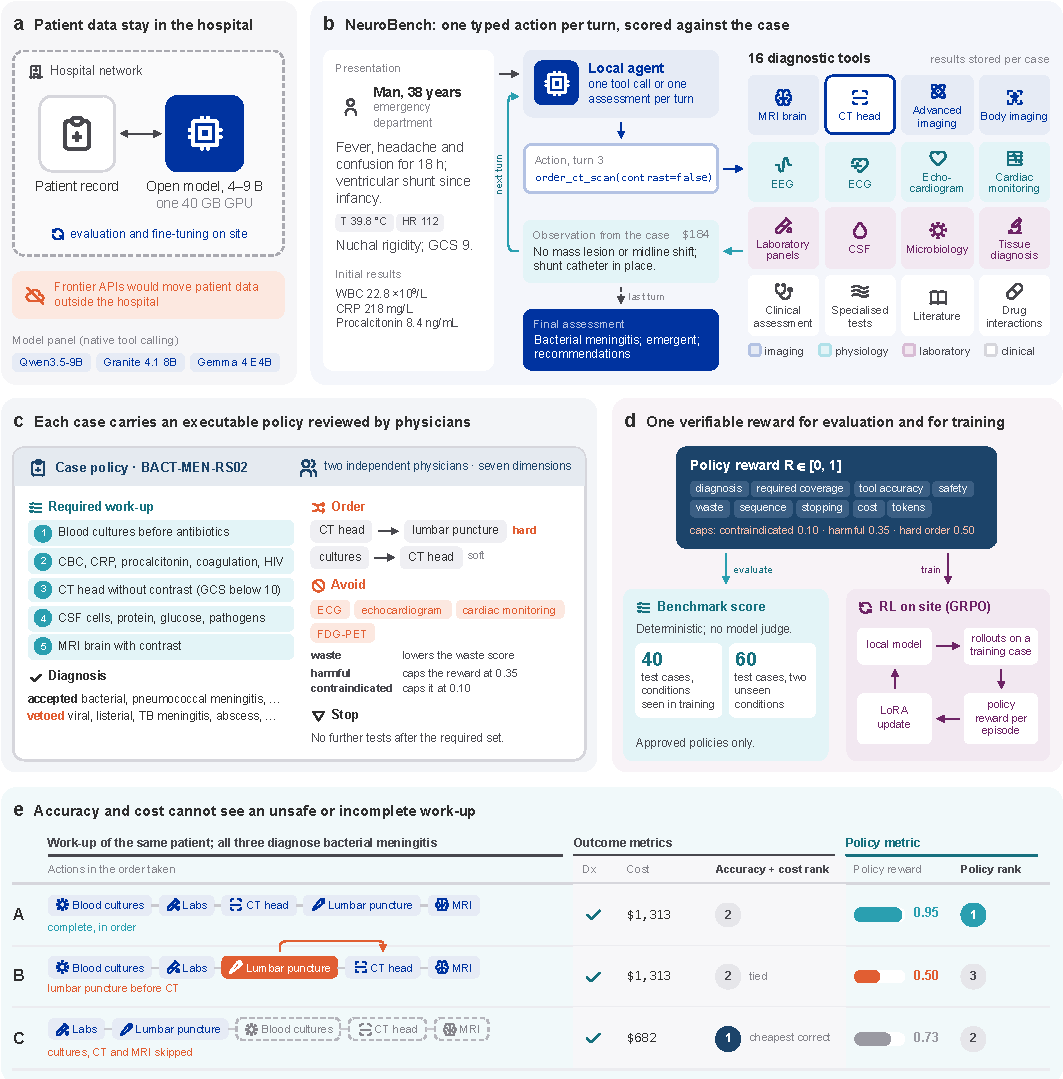
\includegraphics[width=\textwidth]{fig1.pdf}
\caption{\textbf{Draft.} Panels: \textbf{a}, local deployment; \textbf{b}, one typed action
per turn; \textbf{c}, the executable policy; \textbf{d}, the policy reward as metric and RL reward;
\textbf{e}, three work-ups, same diagnosis, opposite rankings. \emph{Why:} the whole thesis in one
figure; panel e is the hook. Legend to write ($\le$250 words), title must state the finding.}
\label{fig:overview}
\end{figure}

\begin{figure}[p]
\centering
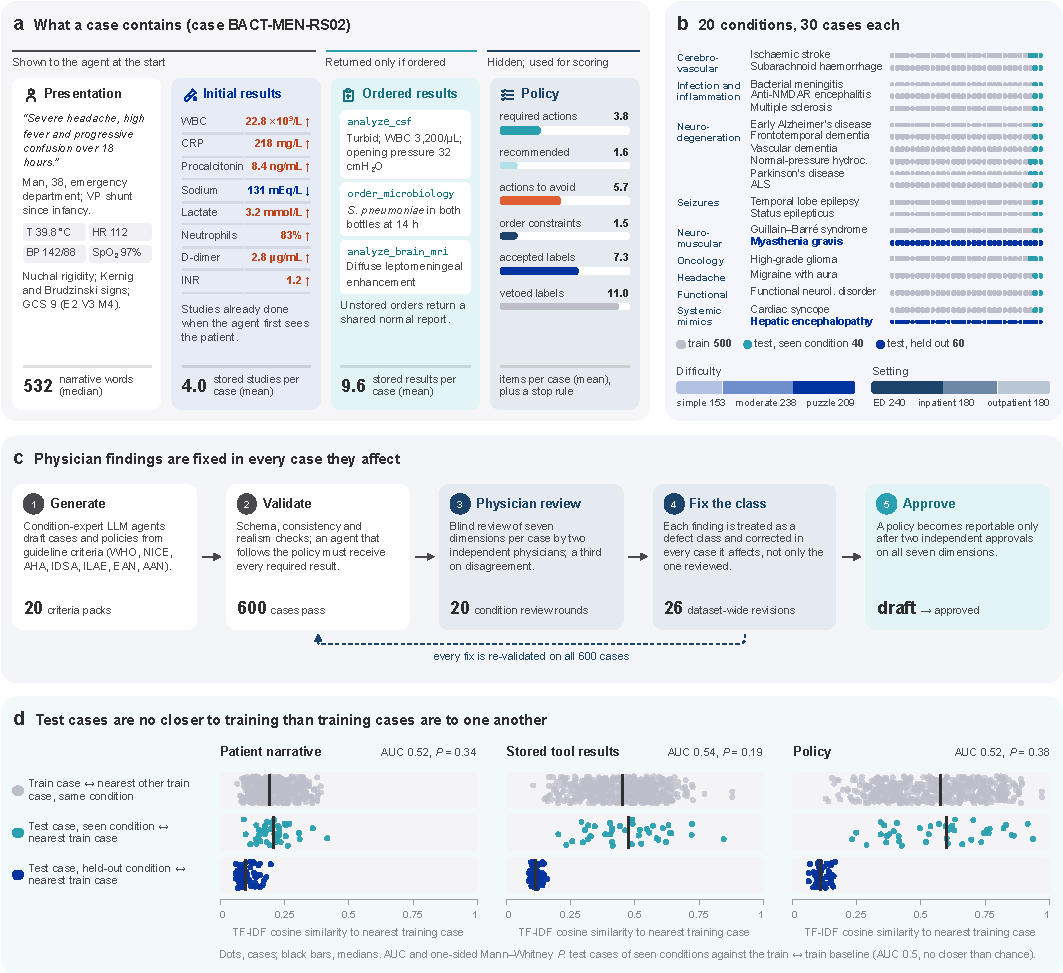
\includegraphics[width=\textwidth]{fig2.pdf}
\caption{\textbf{Draft.} Panels: \textbf{a}, what a case contains (visible, on order, hidden);
\textbf{b}, 20 conditions and the split; \textbf{c}, generation, validation, blind review, defect-class
fixes; \textbf{d}, nearest-neighbour similarity to training for narrative, results and policy.
\emph{Why:} pre-empts the dataset-quality and leakage objections. Legend to write ($\le$250 words).}
\label{fig:benchmark}
\end{figure}

% ---------------------------------------------------------------------------------------------
\subsection{R2. Outcome metrics hide unsafe work-ups and change the ranking of models}\label{sec:outcome}

\role{Claim C1 (E4). Shows the Fig.~1e example at scale: the gap is real and frequent, so training on
the outcome is a problem worth solving.}

\content
\begin{itemize}
\item Panel: Qwen3.5-9B, Granite 4.1 8B, Gemma 4 E4B $\times$ policy / direct / ReAct loops, plus two or
three frontier models.
\item Accuracy and cost vs policy reward per model.
\item Share of correct diagnoses reached with a cap triggered or required actions missing.
\item Rank agreement between outcome and policy rankings (Kendall $\tau$, bootstrap CI).
\end{itemize}

\structure
\begin{enumerate}
\item Claim and setup (80 words).
\item Correct but unsafe: rates per model (150).
\item Rankings change (120).
\item One concrete episode (50).
\end{enumerate}

\artefacts
\begin{itemize}
\item \textbf{Fig.~3}: a, accuracy vs policy reward (one point per model $\times$ loop); b, slope chart of
the two rankings; c, stacked violation types behind correct diagnoses; d, one episode. \emph{Why:}
a and b show mis-ranking, c shows what outcome hides, d makes it concrete.
\item \textbf{ED2} loop ablation: keeps loops out of the main story.
\end{itemize}

\status{To run on the frozen dataset; all earlier baselines predate scorer v2.}

\begin{figure}[p]
\centering
\figplaceholder{Fig.~3 | Outcome metrics vs the policy reward across the panel (E4)}{%
\textbf{a}, accuracy vs mean policy reward, 95\% CIs. \textbf{b}, accuracy+cost ranking vs policy
ranking, Kendall $\tau$. \textbf{c}, violations among correct diagnoses, per model. \textbf{d}, one
episode: correct diagnosis, unsafe path.}
\caption{To design after E4.}
\label{fig:panel}
\end{figure}

% ---------------------------------------------------------------------------------------------
\subsection{R3. Training on the policy reward teaches the work-up without losing accuracy}\label{sec:rl}

\role{Claims C2 and C4 (E1): the causal test of the thesis. Everything else supports this subsection,
so it gets the most words.}

\content
\begin{itemize}
\item Design: base $\to$ SFT $\to$ GRPO with two rewards that differ only in the signal (outcome =
accuracy + cost, SDBench-style; policy). Same models, data, seeds, budget.
\item Approved test split, seen and held-out conditions separately: accuracy, required coverage, safety
violations, cost, number of actions.
\item What the outcome arm learns: shortcuts (skipped cultures or imaging, invasive tests early).
\item Statistics: paired by case; Wilcoxon + paired bootstrap; McNemar for binary outcomes.
\end{itemize}

\structure
\begin{enumerate}
\item Design in two sentences, the two arms (100 words).
\item Main effect on the test split (200).
\item Held-out conditions (120).
\item Learned behaviour, with examples (130).
\item Accuracy is not paid for it; cost and tokens (50).
\end{enumerate}

\artefacts
\begin{itemize}
\item \textbf{Fig.~4}: a, training curves (train-side validation only); b, paired test results for
base, SFT, GRPO-outcome, GRPO-policy; c, same on held-out conditions; d, action sequences of both arms
on one case. \emph{Why:} b is the central number; c answers ``memorised conditions''; d shows the
mechanism (shortcuts vs work-up).
\item \textbf{ED3} seeds and CIs; \textbf{ED4} reward-weight sensitivity: the effect is not a tuning
artefact.
\end{itemize}

\status{To run. July GRPO not reportable (test split used for selection); September runs lack
evaluation and their rollouts sit only on the A100 VM.}

\begin{figure}[p]
\centering
\figplaceholder{Fig.~4 | Outcome reward vs policy reward in RL (E1)}{%
\textbf{a}, training curves of both arms. \textbf{b}, test split, paired per case: accuracy, required
coverage, violations, cost. \textbf{c}, the 60 held-out-condition cases. \textbf{d}, action sequences of
the two arms on one case.}
\caption{To design after E1.}
\label{fig:rl}
\end{figure}

% ---------------------------------------------------------------------------------------------
\subsection{R4. Physicians agree with the policy reward}\label{sec:validity}

\role{Claim C3 (E2). Without it the policy reward is our opinion; NMI reviewers will ask whether the
metric measures what clinicians value.}

\content
\begin{itemize}
\item Blinded rating of a stratified sample of episodes (model and reward hidden), fixed scale for
safety and appropriateness.
\item Spearman $\rho$ of physician scores with policy reward, accuracy+cost and an LLM judge.
\item Inter-rater agreement (Cohen or Fleiss $\kappa$).
\end{itemize}

\structure
\begin{enumerate}
\item Design (100 words).
\item Correlations, policy vs alternatives (170).
\item Agreement and disagreements (80).
\end{enumerate}

\artefacts
\begin{itemize}
\item \textbf{Fig.~5}: a, design; b, $\rho$ for the three scores with CIs; c, $\kappa$. \emph{Why:} b
is the claim; c bounds how much agreement is possible.
\end{itemize}

\status{To design and run; needs physician time. Fix sample size and protocol this week.}

\begin{figure}[p]
\centering
\figplaceholder{Fig.~5 | Blinded physician ratings vs automatic scores (E2)}{%
\textbf{a}, rating design. \textbf{b}, physician score vs policy reward, accuracy+cost, LLM judge
(Spearman $\rho$, CIs). \textbf{c}, inter-rater agreement.}
\caption{To design after E2.}
\label{fig:validity}
\end{figure}

% ---------------------------------------------------------------------------------------------
\subsection{R5. Transfer to real patient records and cost of local deployment}\label{sec:transfer}

\role{Claims C4 and C5 (E3, E5). Answers ``it only works on your simulator'' and makes the local
argument of \P1 concrete.}

\content
\begin{itemize}
\item Trained agents on MIMIC-IV neurology admissions, scored against the guideline policy and compared
with clinicians' recorded orders.
\item Latency, GPU memory and cost per case on one A100 vs frontier APIs.
\end{itemize}

\structure
\begin{enumerate}
\item Cohort and scoring (100 words).
\item Transfer results (180).
\item Deployment cost (120).
\end{enumerate}
\textbf{Fallback:} no MIMIC-IV in time $\Rightarrow$ keep deployment only, transfer becomes future work.

\artefacts
\begin{itemize}
\item \textbf{Fig.~6}: a, MIMIC-IV accuracy and adherence for base, GRPO-outcome, GRPO-policy; b,
overlap of agent orders with the policy and with clinicians; c, latency, memory, cost per case.
\emph{Why:} a and b carry C4 on real data; c carries C5.
\end{itemize}

\status{E3 waits for MIMIC-IV access (requested Oct 2026); E5 can run now.}

\begin{figure}[p]
\centering
\figplaceholder{Fig.~6 | Real records and deployment cost (E3, E5)}{%
\textbf{a}, MIMIC-IV cohort: accuracy and adherence per arm. \textbf{b}, overlap with policy and with
clinicians' orders. \textbf{c}, latency, memory, cost per case, local vs API.}
\caption{To design after E3 and E5.}
\label{fig:transfer}
\end{figure}

% Discussion plan: no subheadings in NMI Articles.

\section{Discussion (700 words, no subheadings)}\label{sec:discussion}

\role{Lift the result from neurology to machine learning (the NMI reader), then disarm the objections
before the reviewers raise them.}

\content
\begin{itemize}
\item The finding in plain words, no numbers repeated.
\item General ML lesson: outcome rewards let agents trade process for answer; an executable process
specification is a cheap, verifiable reward that removes the trade.
\item Clinical lesson: small local models become viable on the right signal; physicians audit
policies, not weights.
\item Limitations stated plainly; outlook.
\end{itemize}

\structure
\noindent{\small
\begin{tabularx}{\linewidth}{@{}>{\raggedright\arraybackslash}p{0.04\linewidth}>{\raggedright\arraybackslash}p{0.20\linewidth}>{\raggedright\arraybackslash}Xr@{}}
\toprule
\P & Move & Points & Words \\ \midrule
1 & Summary & What we built, the central finding & 120 \\
2 & ML meaning & Process vs outcome reward; link to process supervision and reward hacking; where else
  it applies (any domain with written protocols: other specialties, lab work, industrial safety) & 180 \\
3 & Clinical meaning & Local viability; policy as audit trail; review effort moves from model to
  policy & 130 \\
4 & Limitations & Synthetic LLM-drafted cases (mitigated by review, MIMIC-IV); one specialty; one
  guideline view per policy; physician cost of authoring; two reviewers; stored results, not a
  generative simulator; reward weights are a choice (ED4) & 200 \\
5 & Outlook & Policies from hospital pathways; model-assisted, physician-checked authoring;
  prospective evaluation & 70 \\
\bottomrule
\end{tabularx}}

\artefacts
None: no figures. Cite ED4 (weights) and ED7 (robustness) inside \P4 so each limitation points to
its evidence.

\status{Write last, after R1--R5 are fixed.}

% Methods plan: short bold subheadings, written for replication; not counted in the 3,500 words.

\section{Methods ($\sim$3,400 words, thirteen subsections)}\label{sec:methods}

\role{Make every Results number reproducible from this section, the released code and the frozen
dataset; answer the replication and leakage questions so the Results can stay short.}

\content
Thirteen subsections, in the order the pipeline runs: data $\to$ environment $\to$ rewards $\to$
models and training $\to$ evaluation.

\structure
\noindent{\footnotesize
\begin{tabularx}{\linewidth}{@{}>{\raggedright\arraybackslash}p{0.17\linewidth}>{\raggedright\arraybackslash}X>{\raggedright\arraybackslash}p{0.22\linewidth}r>{\raggedright\arraybackslash}p{0.14\linewidth}@{}}
\toprule
Subsection & What goes in & Why & Words & Source \\ \midrule
Cases & Generation from 20 guideline packs; case schema; difficulty and setting mix; frozen version
  and hash & Dataset provenance & 350 & schemas, cases \\
Policies and review & Policy fields; 7 dimensions; blind double review, third on disagreement;
  approval rule; defect-class fixes & Why the policy is trustworthy & 350 & policy\_\allowbreak{}eligibility \\
Environment & Typed loop; 16 tools from the cost registry; schema validation; stored and library
  results; invalid-output budget; forced final turn & Replication of episodes & 300 & harness doc,
  tool contract \\
Policy reward & Components, weights, gating, caps; scorer v2; equation (1) & The object under test
  & 400 & policy\_\allowbreak{}reward \\
Outcome reward & Accuracy + cost as in SDBench, same scorer and costs & The two arms differ only in
  the signal & 150 & --- \\
Models, inference & Panel, versions, vLLM, frozen sampling, seeds; frontier access (synthetic only)
  & Replication & 200 & model\_\allowbreak{}registry \\
SFT & Episode source; LoRA; same transcript codec as inference & No train/inference mismatch & 200
  & train\_\allowbreak{}sft, context \\
RL & GRPO, colocated vLLM, DAPO loss, token-level IS; selection on train-side validation only;
  compute & Central experiment & 350 & train\_\allowbreak{}grpo \\
Split, leakage & 500/100, held-out conditions; test guard; similarity test; release dates; SE-P07
  & Pre-empts contamination & 300 & leakage audit \\
MIMIC-IV & Cohort; records to cases (\texttt{provenance: record}); comparison with clinicians'
  orders; local inference only & External validity, DUA compliance & 250 & --- \\
Rating study & Sampling, blinding, scale, raters, agreement & Validity of C3 & 200 & --- \\
Statistics & Case as unit; Wilcoxon, bootstrap, McNemar, mixed-effects; $\tau$, $\rho$, $\kappa$;
  multiplicity & One place for all tests & 250 & --- \\
Use of LLMs & Case drafting, code and text editing; human review and responsibility & Required by
  NMI & 100 & --- \\
\bottomrule
\end{tabularx}}

\artefacts
\begin{itemize}
\item \textbf{Equation (1)}, the policy reward: the only formula in the paper, so reviewers can check
gating and caps.
\item \textbf{ED Table~1} (tools and costs) and \textbf{ED Table~2} (hyperparameters, compute): keep
long lists out of the text.
\end{itemize}

\status{Can be drafted now from the code, except MIMIC-IV and the rating study.}

% Back matter plan: statements required by Nature Portfolio journals.

\section*{Declarations}

\role{Required statements; data and code availability also carry the release argument of the paper.}

\structure
\noindent{\small
\begin{tabularx}{\linewidth}{@{}>{\raggedright\arraybackslash}p{0.20\linewidth}>{\raggedright\arraybackslash}X>{\raggedright\arraybackslash}p{0.26\linewidth}@{}}
\toprule
Statement & What goes in & Open decision \\ \midrule
Data availability & Benchmark (cases, policies, annotations) with a DOI; MIMIC-IV via PhysioNet DUA
  & Test answers with a canary string, or behind an evaluation server \\
Code availability & Harness, reward, training, evaluation; Zenodo DOI at the paper commit & --- \\
Acknowledgements & Reviewers not authors; CERN compute & --- \\
Funding & Nature Portfolio format & Grant numbers \\
Author contributions & CRediT roles & Author list \\
Competing interests & Statement & --- \\
Ethics & Synthetic cases, no patient data; consent or exemption for review and rating study; MIMIC-IV
  DUA & Check with supervisors \\
\bottomrule
\end{tabularx}}

\status{Decide the test-split release before submission; it also affects the public repository.}

% Extended Data plan: at most 10 items, each cited in the main text.

\section*{Extended Data ($\le$10 items)}

\role{Hold what a reviewer will ask for but the story does not need; each item backs one claim and is
cited where that claim is made.}

\artefacts
\noindent{\small
\begin{tabularx}{\linewidth}{@{}l>{\raggedright\arraybackslash}Xl>{\raggedright\arraybackslash}p{0.20\linewidth}@{}}
\toprule
Item & Content & Backs & Why \\ \midrule
ED1 & Per-condition, per-difficulty results, all models and arms & C1, C2 & Effect not from one
  condition \\
ED2 & Loop ablation: policy, direct, ReAct & C1 & Loops out of main text \\
ED3 & Seed variability and CIs & C2 & Stability \\
ED4 & Sensitivity to reward weights and caps & C2 & Not a tuning artefact \\
ED5 & Scorer v2 vs physician labels & R1 & Diagnosis metric is valid \\
ED6 & Full leakage audit & R1 & Contamination \\
ED7 & Robustness: red herrings, missing results, paraphrases & C2, C4 & Not surface cues \\
ED8 & Shortcuts learned under the outcome reward & C2 & Mechanism \\
ED T1 & Tools, parameters, costs & R1 & Replication \\
ED T2 & Hyperparameters, compute per run & C5, Methods & Replication, cost \\
\bottomrule
\end{tabularx}}

\status{ED5, ED6, ED T1 can be built now; the others follow E1, E4.}

% Supplementary Information plan: a separate PDF at submission.

\section*{Supplementary Information (separate PDF)}

\role{Everything needed to replicate or audit, nothing needed to follow the story.}

\artefacts
\noindent{\small
\begin{tabularx}{\linewidth}{@{}l>{\raggedright\arraybackslash}X>{\raggedright\arraybackslash}p{0.30\linewidth}@{}}
\toprule
Item & Content & Why \\ \midrule
Note 1 & One complete case (BACT-MEN-RS02) with policy and every stored result & Shows the object;
  same case as Fig.~1e \\
Note 2 & Policy schema, diagnosis synonym rules & Audit of the reward \\
Note 3 & System prompts and tool schemas as sent & Replication \\
Note 4 & Case-generation prompts, criteria packs & Provenance of synthetic cases \\
Note 5 & Review protocol and form; rating-study protocol & Validity of C3 and of approvals \\
Data & Per-case, per-episode results; source data for every figure & Required by Nature \\
\bottomrule
\end{tabularx}}


\bibliography{references}

\end{document}
